%%%%%%%%%%%%%%%%%%%%%%%%%%%%%%%%%%%%%%%%%%%%%%%%%%%%%%%%%%%%%%%%%%%%%%%%%%%%%
% Chapter 6: Ampliación de funcionalidades
%%%%%%%%%%%%%%%%%%%%%%%%%%%%%%%%%%%%%%%%%%%%%%%%%%%%%%%%%%%%%%%%%%%%%%%%%%%%%%%

%++++++++++++++++++++++++++++++++++++++++++++++++++++++++++++++++++++++++++++++

En este proyecto de fin de grado se han realizado cuatro ampliaciones sobre las funcionalidades originales 
del simulador. 


%++++++++++++++++++++++++++++++++++++++++++++++++++++++++++++++++++++++++++++++
\section{Parseador}
\label{6:sec1}

Una de las características más deseadas por parte de los usuarios de SIMDE 
(entre los que yo mismo me puedo incluir), es un sistema de errores más descriptivo. 

Por desgracia, en la versión original de SIMDE sólo se mostraba una notificación que indicaba
que el código cargado contenía errores.

\begin{figure}[!th]
\begin{center}
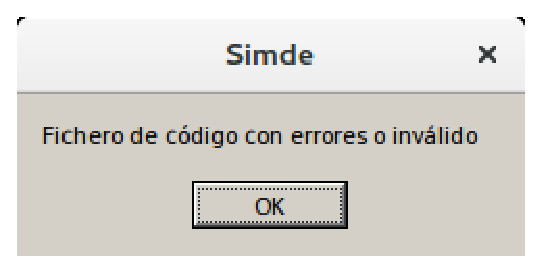
\includegraphics[width=0.5\textwidth]{images/cap6/errorsimde.eps}
\caption{Notificacion de error original SIMDE}
\end{center}
\end{figure}

Ahora, tras una serie de modificaciones en el parseados de código, se muestran los siguientes errores:

\begin{enumerate}
\item Operando erróneo
\item Opcode desconocido
\item Etiqueta repetida
\end{enumerate}

Además, se muestra la línea del error. Esto resulta tremendamente importante, 
ya que una de las aplicaciones de SIMDE requiere realizar mejoras en el rendimiento
de código haciendo uso de técnicas como el desenrollado de bucles, 
dando lugar a códigos de considerable tamaño.


\begin{figure}[!th]
\begin{center}
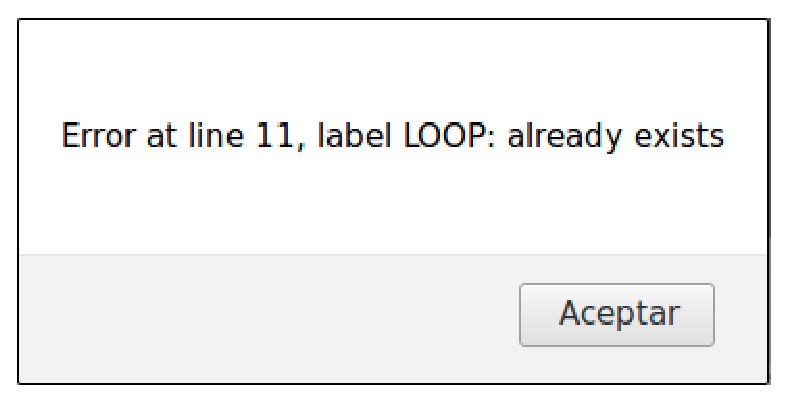
\includegraphics[width=0.5\textwidth]{images/cap6/nuevoerrorsimde.eps}
\caption{Ejemplos de errores en la nueva versión de simde}
\end{center}
\end{figure}

%++++++++++++++++++++++++++++++++++++++++++++++++++++++++++++++++++++++++++++++
\section{Modo de ejecución en lotes}
\label{6:sec2}

Otra característica que habría sido resultado muy deseable por mi parte y por parte de mis compañeros, 
es no tener el limite de velocidad que tiene la versión original.

En mi caso, la cantidad media de ciclos de los ejercicios que se me propusieron superaba los 500 ciclos,
 haciendo un tiempo medio de ejecución de 2 - 3 minutos, lo cual sumado a 
la media de pruebas, a la depuración de errores, y a las distintas optimizaciones, 
alargaba de forma innecesaria el desarrollo de los ejercicios.

Es por eso que ahora, cuando el campo de velocidad está en 0, se ejecuta la simulación a velocidad 
máxima, y solo se refresca la interfaz cuando termina la ejecución. Ahorrando así 
recursos. 

%++++++++++++++++++++++++++++++++++++++++++++++++++++++++++++++++++++++++++++++
\section{Histórico}
\label{6:sec3}

Otra característica que resultaba necesaria en el simulador y que se añoraba sobre todo en el primer
contacto era la posibilidad de ir hacia atrás.

\bigskip
En un principio, se esperaba utilizar algún sistema gestor de estados y permitir el time traveling. 
Por desgracia debido al volumen de este trabajo de fin de grado decidió no utilizarse este tipo de 
soluciones.

\bigskip
Sin embargo, la idea del \textit{time traveling} resultaba más que deseable, por lo que se implementó
de una forma un tanto rústica. Para permitir emular este comportamiento y mantener la fidelidad de 
la ejecución (recordemos que existen una serie de operaciones que son sujetas a un porcentaje de fallos
aleatorios), lo que se hizo fue acumular el estado visual de la máquina, el modelo en sí con el 
que se dibujaban los componentes.

\bigskip
De tal forma, cuando un usuario entraba en este modo timetraveling recorre un array de estados de la 
interfaz, imprimiendo la información almacenada, sin afectar al comportamiento de la máquina, pero 
emulando ese \textit{time traveling} de cara al usuario.

\bigskip
Por tanto, se considera que un usuario que retroceda X pasos, deberá avanzar esos X pasos para continuar
la ejecución (o en su defecto, pulsar el botón \textbf{Play}). Esto es así porque aunque como repito, se 
trata de una característica enormemente deseada en la primera toma de contacto del simulador, no se trata
de una característica de la que se espere que el usuario abuse.
